% Options for packages loaded elsewhere
\PassOptionsToPackage{unicode}{hyperref}
\PassOptionsToPackage{hyphens}{url}
%
\documentclass[
]{article}
\usepackage{amsmath,amssymb}
\usepackage{lmodern}
\usepackage{iftex}
\ifPDFTeX
  \usepackage[T1]{fontenc}
  \usepackage[utf8]{inputenc}
  \usepackage{textcomp} % provide euro and other symbols
\else % if luatex or xetex
  \usepackage{unicode-math}
  \defaultfontfeatures{Scale=MatchLowercase}
  \defaultfontfeatures[\rmfamily]{Ligatures=TeX,Scale=1}
\fi
% Use upquote if available, for straight quotes in verbatim environments
\IfFileExists{upquote.sty}{\usepackage{upquote}}{}
\IfFileExists{microtype.sty}{% use microtype if available
  \usepackage[]{microtype}
  \UseMicrotypeSet[protrusion]{basicmath} % disable protrusion for tt fonts
}{}
\makeatletter
\@ifundefined{KOMAClassName}{% if non-KOMA class
  \IfFileExists{parskip.sty}{%
    \usepackage{parskip}
  }{% else
    \setlength{\parindent}{0pt}
    \setlength{\parskip}{6pt plus 2pt minus 1pt}}
}{% if KOMA class
  \KOMAoptions{parskip=half}}
\makeatother
\usepackage{xcolor}
\usepackage[margin=1in]{geometry}
\usepackage{color}
\usepackage{fancyvrb}
\newcommand{\VerbBar}{|}
\newcommand{\VERB}{\Verb[commandchars=\\\{\}]}
\DefineVerbatimEnvironment{Highlighting}{Verbatim}{commandchars=\\\{\}}
% Add ',fontsize=\small' for more characters per line
\usepackage{framed}
\definecolor{shadecolor}{RGB}{248,248,248}
\newenvironment{Shaded}{\begin{snugshade}}{\end{snugshade}}
\newcommand{\AlertTok}[1]{\textcolor[rgb]{0.94,0.16,0.16}{#1}}
\newcommand{\AnnotationTok}[1]{\textcolor[rgb]{0.56,0.35,0.01}{\textbf{\textit{#1}}}}
\newcommand{\AttributeTok}[1]{\textcolor[rgb]{0.77,0.63,0.00}{#1}}
\newcommand{\BaseNTok}[1]{\textcolor[rgb]{0.00,0.00,0.81}{#1}}
\newcommand{\BuiltInTok}[1]{#1}
\newcommand{\CharTok}[1]{\textcolor[rgb]{0.31,0.60,0.02}{#1}}
\newcommand{\CommentTok}[1]{\textcolor[rgb]{0.56,0.35,0.01}{\textit{#1}}}
\newcommand{\CommentVarTok}[1]{\textcolor[rgb]{0.56,0.35,0.01}{\textbf{\textit{#1}}}}
\newcommand{\ConstantTok}[1]{\textcolor[rgb]{0.00,0.00,0.00}{#1}}
\newcommand{\ControlFlowTok}[1]{\textcolor[rgb]{0.13,0.29,0.53}{\textbf{#1}}}
\newcommand{\DataTypeTok}[1]{\textcolor[rgb]{0.13,0.29,0.53}{#1}}
\newcommand{\DecValTok}[1]{\textcolor[rgb]{0.00,0.00,0.81}{#1}}
\newcommand{\DocumentationTok}[1]{\textcolor[rgb]{0.56,0.35,0.01}{\textbf{\textit{#1}}}}
\newcommand{\ErrorTok}[1]{\textcolor[rgb]{0.64,0.00,0.00}{\textbf{#1}}}
\newcommand{\ExtensionTok}[1]{#1}
\newcommand{\FloatTok}[1]{\textcolor[rgb]{0.00,0.00,0.81}{#1}}
\newcommand{\FunctionTok}[1]{\textcolor[rgb]{0.00,0.00,0.00}{#1}}
\newcommand{\ImportTok}[1]{#1}
\newcommand{\InformationTok}[1]{\textcolor[rgb]{0.56,0.35,0.01}{\textbf{\textit{#1}}}}
\newcommand{\KeywordTok}[1]{\textcolor[rgb]{0.13,0.29,0.53}{\textbf{#1}}}
\newcommand{\NormalTok}[1]{#1}
\newcommand{\OperatorTok}[1]{\textcolor[rgb]{0.81,0.36,0.00}{\textbf{#1}}}
\newcommand{\OtherTok}[1]{\textcolor[rgb]{0.56,0.35,0.01}{#1}}
\newcommand{\PreprocessorTok}[1]{\textcolor[rgb]{0.56,0.35,0.01}{\textit{#1}}}
\newcommand{\RegionMarkerTok}[1]{#1}
\newcommand{\SpecialCharTok}[1]{\textcolor[rgb]{0.00,0.00,0.00}{#1}}
\newcommand{\SpecialStringTok}[1]{\textcolor[rgb]{0.31,0.60,0.02}{#1}}
\newcommand{\StringTok}[1]{\textcolor[rgb]{0.31,0.60,0.02}{#1}}
\newcommand{\VariableTok}[1]{\textcolor[rgb]{0.00,0.00,0.00}{#1}}
\newcommand{\VerbatimStringTok}[1]{\textcolor[rgb]{0.31,0.60,0.02}{#1}}
\newcommand{\WarningTok}[1]{\textcolor[rgb]{0.56,0.35,0.01}{\textbf{\textit{#1}}}}
\usepackage{graphicx}
\makeatletter
\def\maxwidth{\ifdim\Gin@nat@width>\linewidth\linewidth\else\Gin@nat@width\fi}
\def\maxheight{\ifdim\Gin@nat@height>\textheight\textheight\else\Gin@nat@height\fi}
\makeatother
% Scale images if necessary, so that they will not overflow the page
% margins by default, and it is still possible to overwrite the defaults
% using explicit options in \includegraphics[width, height, ...]{}
\setkeys{Gin}{width=\maxwidth,height=\maxheight,keepaspectratio}
% Set default figure placement to htbp
\makeatletter
\def\fps@figure{htbp}
\makeatother
\setlength{\emergencystretch}{3em} % prevent overfull lines
\providecommand{\tightlist}{%
  \setlength{\itemsep}{0pt}\setlength{\parskip}{0pt}}
\setcounter{secnumdepth}{-\maxdimen} % remove section numbering
\ifLuaTeX
  \usepackage{selnolig}  % disable illegal ligatures
\fi
\IfFileExists{bookmark.sty}{\usepackage{bookmark}}{\usepackage{hyperref}}
\IfFileExists{xurl.sty}{\usepackage{xurl}}{} % add URL line breaks if available
\urlstyle{same} % disable monospaced font for URLs
\hypersetup{
  pdftitle={High dimensioanl simulation study},
  hidelinks,
  pdfcreator={LaTeX via pandoc}}

\title{High dimensioanl simulation study}
\author{}
\date{\vspace{-2.5em}}

\begin{document}
\maketitle

\begin{Shaded}
\begin{Highlighting}[]
\NormalTok{N }\OtherTok{=} \DecValTok{2000}
\NormalTok{n }\OtherTok{=} \DecValTok{200}
\NormalTok{BIAS\_res }\OtherTok{=} \ConstantTok{NULL}
\NormalTok{SE\_res }\OtherTok{=} \ConstantTok{NULL}
\NormalTok{pvec }\OtherTok{=} \DecValTok{1}\SpecialCharTok{:}\DecValTok{18} \SpecialCharTok{*} \DecValTok{10}

\NormalTok{X\_whole }\OtherTok{=} \FunctionTok{matrix}\NormalTok{(}\FunctionTok{rnorm}\NormalTok{(N }\SpecialCharTok{*} \DecValTok{500}\NormalTok{, }\DecValTok{2}\NormalTok{, }\DecValTok{1}\NormalTok{), }\AttributeTok{nr =}\NormalTok{ N, }\AttributeTok{nc =} \DecValTok{500}\NormalTok{)}

\ControlFlowTok{for}\NormalTok{(p }\ControlFlowTok{in}\NormalTok{ pvec)\{}
  \CommentTok{\# p = 10}
  \FunctionTok{set.seed}\NormalTok{(}\DecValTok{1}\NormalTok{)}
  \FunctionTok{print}\NormalTok{(p)}
\NormalTok{s }\OtherTok{=} \DecValTok{5}

\NormalTok{X }\OtherTok{=}\NormalTok{ X\_whole[,}\DecValTok{1}\SpecialCharTok{:}\NormalTok{p]}
\NormalTok{beta }\OtherTok{=} \FunctionTok{c}\NormalTok{(}\FunctionTok{rep}\NormalTok{(}\DecValTok{1}\NormalTok{, s), }\FunctionTok{rep}\NormalTok{(}\DecValTok{0}\NormalTok{, p }\SpecialCharTok{{-}}\NormalTok{ s))}
\NormalTok{e }\OtherTok{=} \FunctionTok{rnorm}\NormalTok{(N, }\DecValTok{0}\NormalTok{, }\DecValTok{1}\NormalTok{)}
\NormalTok{y }\OtherTok{=}\NormalTok{ X }\SpecialCharTok{\%*\%}\NormalTok{ beta }\SpecialCharTok{+}\NormalTok{ e}
\NormalTok{t\_y }\OtherTok{=} \FunctionTok{sum}\NormalTok{(y)}

\CommentTok{\# pi1 = X[,1]\^{}2 / sum(X[,1]\^{}2) * n}
\NormalTok{pi1 }\OtherTok{=} \FunctionTok{rep}\NormalTok{(n }\SpecialCharTok{/}\NormalTok{ N, N)}
\NormalTok{d1 }\OtherTok{=} \DecValTok{1} \SpecialCharTok{/}\NormalTok{ pi1}

\NormalTok{res }\OtherTok{=} \ConstantTok{NULL}
\NormalTok{res2 }\OtherTok{=} \ConstantTok{NULL}
\NormalTok{res3 }\OtherTok{=} \ConstantTok{NULL}
\NormalTok{SIMNUM }\OtherTok{=} \DecValTok{500}
\ControlFlowTok{for}\NormalTok{(simnum }\ControlFlowTok{in} \DecValTok{1}\SpecialCharTok{:}\NormalTok{SIMNUM)\{}
  \CommentTok{\# set.seed(simnum)}
\NormalTok{  Index }\OtherTok{=} \FunctionTok{sample}\NormalTok{(}\DecValTok{1}\SpecialCharTok{:}\NormalTok{N, }\AttributeTok{size =}\NormalTok{ n, }\AttributeTok{replace =} \ConstantTok{FALSE}\NormalTok{, }\AttributeTok{prob =}\NormalTok{ pi1)}
\NormalTok{  y\_s }\OtherTok{=}\NormalTok{ y[Index]}
\NormalTok{  X\_s }\OtherTok{=}\NormalTok{ X[Index, ]}
\NormalTok{  d1\_s }\OtherTok{=}\NormalTok{ d1[Index]}
\NormalTok{  lm\_obj }\OtherTok{=} \FunctionTok{lm}\NormalTok{(y\_s }\SpecialCharTok{\textasciitilde{}}\NormalTok{  X\_s, }\AttributeTok{weights =}\NormalTok{ d1\_s)}
\NormalTok{  beta\_hat }\OtherTok{=}\NormalTok{ lm\_obj}\SpecialCharTok{$}\NormalTok{coefficients[}\SpecialCharTok{{-}}\DecValTok{1}\NormalTok{]}
  \CommentTok{\#drop(solve(t(X\_s) \%*\% diag(d1\_s) \%*\% X\_s, t(X\_s) \%*\% diag(d1\_s) \%*\% y\_s))}
  
  \CommentTok{\# beta\_hat = unname(lm(y\_s \textasciitilde{}  t(apply(X\_s, 1, function(k) k }
  \CommentTok{\# {-} colSums(X\_s * d1\_s) / N)), weights = d1\_s)$coefficients[{-}1])}
  
\NormalTok{  y\_HT }\OtherTok{=} \FunctionTok{sum}\NormalTok{(y\_s }\SpecialCharTok{*}\NormalTok{ d1\_s)}
  
\NormalTok{  y\_diff }\OtherTok{=} \FunctionTok{drop}\NormalTok{(}\FunctionTok{colSums}\NormalTok{(X) }\SpecialCharTok{\%*\%}\NormalTok{ beta }\SpecialCharTok{+} \FunctionTok{sum}\NormalTok{((y\_s }\SpecialCharTok{{-}} \FunctionTok{drop}\NormalTok{(X\_s }\SpecialCharTok{\%*\%}\NormalTok{ beta)) }\SpecialCharTok{*}\NormalTok{ d1\_s))}
  
\NormalTok{  y\_GREG }\OtherTok{=} \FunctionTok{drop}\NormalTok{(}\FunctionTok{colSums}\NormalTok{(X) }\SpecialCharTok{\%*\%}\NormalTok{ beta\_hat }\SpecialCharTok{+} \FunctionTok{sum}\NormalTok{((y\_s }\SpecialCharTok{{-}} \FunctionTok{drop}\NormalTok{(X\_s }\SpecialCharTok{\%*\%}\NormalTok{ beta\_hat)) }\SpecialCharTok{*}\NormalTok{ d1\_s))}
  
\NormalTok{  y\_model }\OtherTok{=} \FunctionTok{drop}\NormalTok{(}\FunctionTok{colSums}\NormalTok{(X) }\SpecialCharTok{\%*\%}\NormalTok{ beta\_hat)}

  \CommentTok{\# sigma\_Debiased = sqrt(drop(t(e\_s)  \%*\% Omega \%*\% e\_s * N\^{}2 / n\^{}2))}
  
\NormalTok{  res }\OtherTok{=} \FunctionTok{rbind}\NormalTok{(res, }\FunctionTok{c}\NormalTok{(}\AttributeTok{HT =}\NormalTok{ y\_HT, }\AttributeTok{Diff =}\NormalTok{ y\_diff, }\AttributeTok{GREG =}\NormalTok{ y\_GREG))}

  
\NormalTok{\}}

\NormalTok{BIAS }\OtherTok{=} \FunctionTok{colMeans}\NormalTok{(res }\SpecialCharTok{{-}}\NormalTok{ t\_y)}
\NormalTok{SE }\OtherTok{=} \FunctionTok{apply}\NormalTok{(res, }\DecValTok{2}\NormalTok{, }\ControlFlowTok{function}\NormalTok{(x) }\FunctionTok{sqrt}\NormalTok{(}\FunctionTok{var}\NormalTok{(x) }\SpecialCharTok{*}\NormalTok{ (}\FunctionTok{length}\NormalTok{(x)}\SpecialCharTok{{-}}\DecValTok{1}\NormalTok{)}\SpecialCharTok{/}\FunctionTok{length}\NormalTok{(x) ))}
\NormalTok{RMSE }\OtherTok{=} \FunctionTok{apply}\NormalTok{(res }\SpecialCharTok{{-}}\NormalTok{ t\_y, }\DecValTok{2}\NormalTok{, }\ControlFlowTok{function}\NormalTok{(x) }\FunctionTok{sqrt}\NormalTok{(}\FunctionTok{mean}\NormalTok{(x}\SpecialCharTok{\^{}}\DecValTok{2}\NormalTok{)))}

\FunctionTok{cbind}\NormalTok{(BIAS, SE, RMSE)}

\NormalTok{BIAS\_res }\OtherTok{=} \FunctionTok{rbind}\NormalTok{(BIAS\_res, BIAS)}
\NormalTok{SE\_res }\OtherTok{=} \FunctionTok{rbind}\NormalTok{(SE\_res, SE)}
\NormalTok{\}}
\end{Highlighting}
\end{Shaded}

\begin{verbatim}
## [1] 10
## [1] 20
## [1] 30
## [1] 40
## [1] 50
## [1] 60
## [1] 70
## [1] 80
## [1] 90
## [1] 100
## [1] 110
## [1] 120
## [1] 130
## [1] 140
## [1] 150
## [1] 160
## [1] 170
## [1] 180
\end{verbatim}

\begin{Shaded}
\begin{Highlighting}[]
\FunctionTok{plot}\NormalTok{(pvec, SE\_res[,}\DecValTok{3}\NormalTok{], }\AttributeTok{type =} \StringTok{"l"}\NormalTok{, }\AttributeTok{col =} \DecValTok{1}\NormalTok{, }\AttributeTok{ylim =} \FunctionTok{c}\NormalTok{(}\FunctionTok{min}\NormalTok{(BIAS\_res), }\FunctionTok{max}\NormalTok{(SE\_res)), }\AttributeTok{main =} \FunctionTok{sprintf}\NormalTok{(}\StringTok{"n = \%g"}\NormalTok{, n), }\AttributeTok{xlab =} \StringTok{"p"}\NormalTok{, }\AttributeTok{ylab =} \StringTok{" "}\NormalTok{)}
\FunctionTok{points}\NormalTok{(pvec, SE\_res[,}\DecValTok{2}\NormalTok{], }\AttributeTok{type =} \StringTok{"l"}\NormalTok{, }\AttributeTok{col =} \DecValTok{2}\NormalTok{)}
\FunctionTok{points}\NormalTok{(pvec, SE\_res[,}\DecValTok{1}\NormalTok{], }\AttributeTok{type =} \StringTok{"l"}\NormalTok{, }\AttributeTok{col =} \DecValTok{4}\NormalTok{)}
\FunctionTok{legend}\NormalTok{(}\StringTok{"topleft"}\NormalTok{, }\FunctionTok{c}\NormalTok{(}\StringTok{"GREG"}\NormalTok{, }\StringTok{"Diff"}\NormalTok{, }\StringTok{"HT"}\NormalTok{), }\AttributeTok{col =} \FunctionTok{c}\NormalTok{(}\DecValTok{1}\NormalTok{,}\DecValTok{2}\NormalTok{,}\DecValTok{4}\NormalTok{), }\AttributeTok{lty =} \DecValTok{1}\NormalTok{, }\AttributeTok{title =} \StringTok{"SE"}\NormalTok{)}

\FunctionTok{points}\NormalTok{(pvec, BIAS\_res[,}\DecValTok{3}\NormalTok{], }\AttributeTok{type =} \StringTok{"l"}\NormalTok{, }\AttributeTok{col =} \DecValTok{1}\NormalTok{, }\AttributeTok{lty =} \DecValTok{2}\NormalTok{)}
\FunctionTok{points}\NormalTok{(pvec, BIAS\_res[,}\DecValTok{2}\NormalTok{], }\AttributeTok{type =} \StringTok{"l"}\NormalTok{, }\AttributeTok{col =} \DecValTok{2}\NormalTok{, }\AttributeTok{lty =} \DecValTok{2}\NormalTok{)}
\FunctionTok{points}\NormalTok{(pvec, BIAS\_res[,}\DecValTok{1}\NormalTok{], }\AttributeTok{type =} \StringTok{"l"}\NormalTok{, }\AttributeTok{col =} \DecValTok{4}\NormalTok{, }\AttributeTok{lty =} \DecValTok{2}\NormalTok{)}
\FunctionTok{legend}\NormalTok{(}\StringTok{"bottomleft"}\NormalTok{, }\FunctionTok{c}\NormalTok{(}\StringTok{"GREG"}\NormalTok{, }\StringTok{"Diff"}\NormalTok{, }\StringTok{"HT"}\NormalTok{), }\AttributeTok{col =} \FunctionTok{c}\NormalTok{(}\DecValTok{1}\NormalTok{,}\DecValTok{2}\NormalTok{,}\DecValTok{4}\NormalTok{), }\AttributeTok{lty =} \DecValTok{2}\NormalTok{, }\AttributeTok{title =} \StringTok{"BIAS"}\NormalTok{)}
\end{Highlighting}
\end{Shaded}

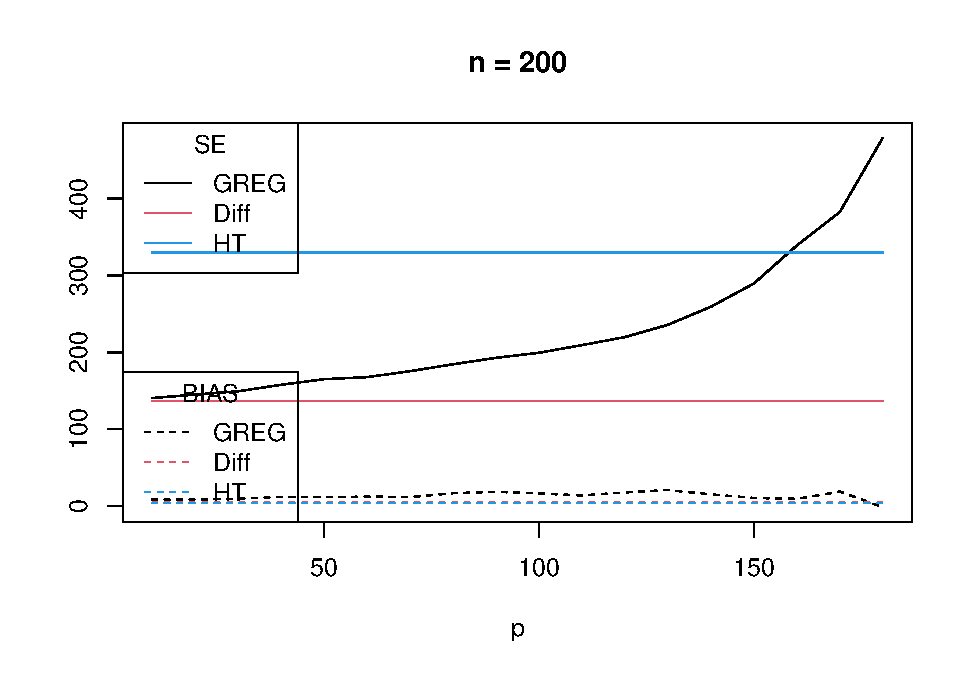
\includegraphics{sim_092622_files/figure-latex/unnamed-chunk-1-1.pdf}

\end{document}
